\subsection{Das Gabor-Wavelet}
\rhead{Gabor-Wavelet}
\begin{figure}
	\centering
	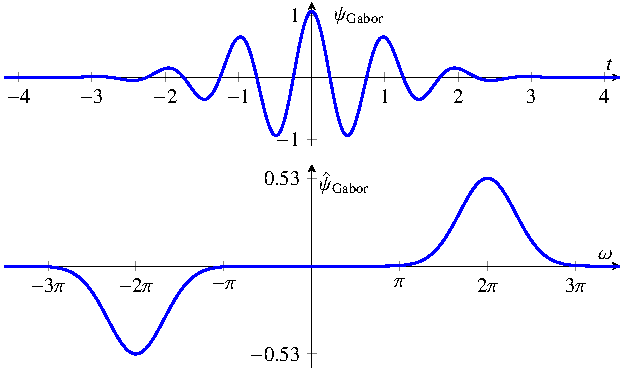
\includegraphics{papers/complex/images/gabor.pdf}
	\caption{Das Gabor-Wavelet für $\sigma = 2\pi$ \label{complex:gabor}}
\end{figure}

Die schlechte Lokalisierung des Haar-Wavelets in der Frequenz ist schon in seinem Spektrum ersichtlich.
Die Frequenzen neben $\omega_\psi$ fallen nur langsam ab.
Durch Heisenberg (Satz~\ref{satz:heisenberg}) wissen wir, dass die beste Lokalisierung durch Gauss-Funktionen erreicht wird.
Als nächstes verwenden wir deshalb das Gabor-Wavelet
\[
	\psi_\text{Gabor} = c_\sigma e^{-\frac{t^2}{2}}\left(\cos\left(\sigma t\right) - \kappa_\sigma\right),
\]
welches in Abbildung~\ref{complex:gabor} ersichtlich ist.
$c_\sigma$ und $\kappa_\sigma$ sind hierbei positive, reelle Konstanten.
$c_\sigma$ korrigiert die Norm des Wavelets, so dass $\|\psi\| = 1$.
$\kappa_\sigma$ ist notwendig für die Zulässigkeitsbedingung~\eqref{cwt:zulaessig}, welche u.~a.~fordert, dass das Integral des Wavelets verschwindet,  $\int_{-\infty}^{\infty}\psi\,\mathrm{d}t = 0$.
$\kappa_\sigma$ ist typischerweise sehr klein und wird in der Numerik oftmals einfach weggelassen.

$\sigma$ erlaubt es, Zeit- und Frequenz-Lokalisierung gegeneinander abzuwägen.
Die dominante Frequenz $\omega_\psi$ dieses Wavelets ist für $5 < \sigma \approx \omega_\psi$.
Das Gabor-Wavelet eignet sich deshalb besonders gut, um einzelne Frequenzen in einem Signal zu finden.
Betrachten wir die Wavelet-Transformierten unserer Beispielsignale mit dem Gabor-Wavelet in Abbildung~\ref{complex:gabor-ex}.

\begin{figure}
	\centering
	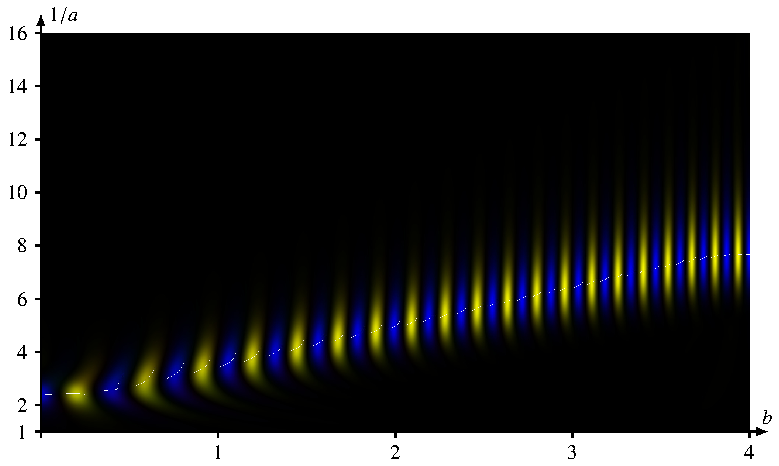
\includegraphics{papers/complex/images/chirp_gabor.pdf}
	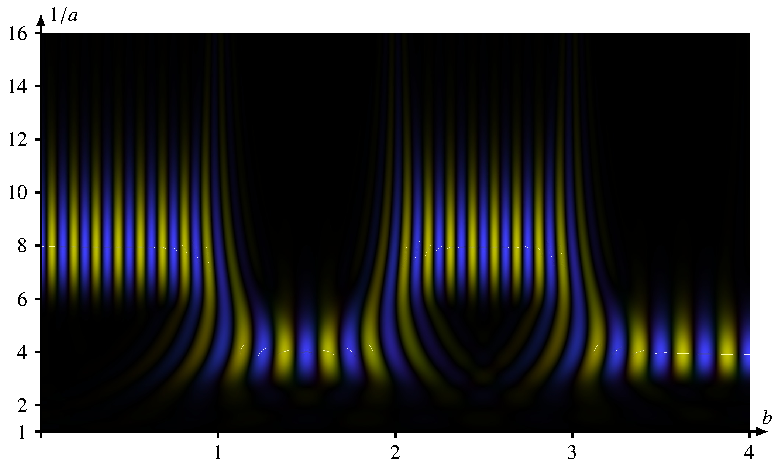
\includegraphics{papers/complex/images/square_gabor.pdf}
	\caption{Wavelet-Transformationen der beiden Beispielsignale mit dem Gabor-Wavelet.
		Die Frequenzlokalisierung ist deutlich besser, aber die Maxima $a_\text{max}(b)$ sind weniger exakt. Zudem ist der Zeitpunkt der Frequenz-Änderung nicht mehr so scharf erkennbar wie beim Haar-Wavelet.}
	\label{complex:gabor-ex}
\end{figure}

Auch hier ist die Signalfrequenz als Schwingung in der Amplitude ersichtlich. 
Die Lokalisierung in der Frequenz ist deutlich besser und die Verschiebung zwischen $a$ und $f$ klein, allerdings fliessen die Frequenzsprünge ineinander über, statt wie beim Haar-Wavelet scharf getrennt zu sein.
Durch die Wahl von $\sigma$ kann die Form des Wavelets angepasst werden und bietet folglich etwas Freiheit.
Wie auch beim Haar-Wavelet ist die Phase und die Amplitude nicht separierbar.
Auch hier finden wir die charakteristische Schwingung in der Amplitude wieder.
Diesem Problem wenden wir uns nun zu.